\chapter{Theoretical Background}
\label{cha:theory}

This chapter describes relevant theory for solving the heading estimation problem.
In order to estimate a vehicle's heading, we must track its movement, \ie perform \textit{target tracking} of the vehicle.
Target tracking is the task of tracking targets, objects of interest, given measurements, outputs from sensors, with different variations of uncertainty.
The camera system is used to detect and input measurements to a filter which process the measurements and predicts the movement of the vehicle.
When using a camera system, it is necessary to use different coordinate systems in order to separate the image information from world information.

\section{General Target Tracking}
The main objective of target tracking is to estimate the states of a target, given measurements or observations from one or more sensors.
A target can be any object for which we are interested in estimating \eg the position, velocity, acceleration, orientation etc.
A \textit{track} is a confirmed target, \ie a target that has been associated with a number of measurements under a certain time.
When performing target tracking, one can be interested in tracking just a single object or tracking multiple objects at the same time.
These two cases are referred to as single-target tracking (\abbrSTT) and multiple-target tracking (\abbrMTT) \cite{Blackman:1999}.
A typical flow chart of a \abbrMTT system can be seen in \Figureref{fig:trackingflowchart}.
Each stage of the procedure in \Figureref{fig:trackingflowchart} is described in detail in \Tableref{tab:trackingflowchart}.
When tracking only a single object, the gating and measurement association are simplified compared to \abbrMTT.

\begin{figure}[!ht]
	\centering
	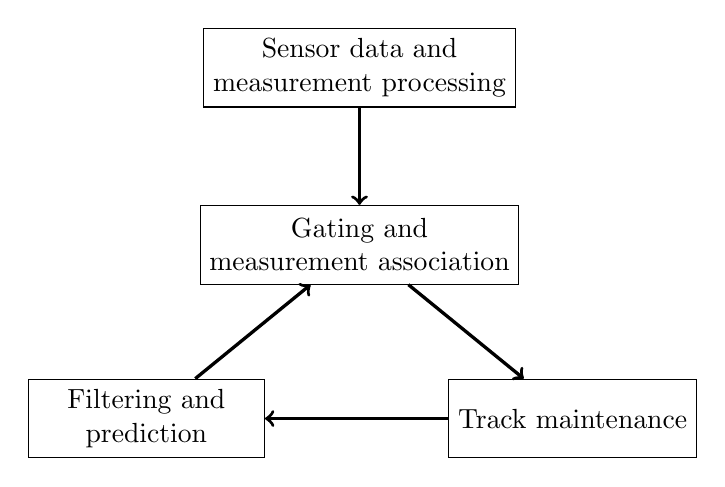
\begin{tikzpicture}
		\tikzstyle{elem} = [rectangle, minimum width = 3cm, minimum height=1cm, align=center, draw=black]

		\node (sensorData) [elem] {Sensor data and \\ measurement processing};
		\node (gatingAssociation) [elem, below of=sensorData, yshift=-1.25cm] {Gating and \\ measurement association};
		\node (trackMaintenance) [elem, below right of=gatingAssociation, yshift=-1.5cm, xshift=2cm] {Track maintenance};
		\node (filter) [elem, below left of=gatingAssociation,  yshift=-1.5cm, xshift=-2cm] {Filtering and \\ prediction};

		\draw [->,very thick] (sensorData) -- (gatingAssociation);
		\draw [->,very thick] (gatingAssociation) -- (trackMaintenance);
		\draw [->,very thick] (trackMaintenance) -- (filter);
		\draw [->,very thick] (filter) -- (gatingAssociation);
	\end{tikzpicture}
	\caption{\label{fig:trackingflowchart} A flow chart of a typical \abbrMTT system.}
\end{figure}

\begin{table}[!ht]
	\centering
	\caption{\label{tab:trackingflowchart} Description of each stage of the \abbrMTT system.}
	\begin{tabular}{|>{\centering\arraybackslash}p{4cm}|p{8cm}|}
		\hline
		\textbf{Stage} & \textbf{Description} \\
		\hline
		Sensor data and measurement processing & External sensors input data to the tracking system. The data might have to be pre-processed. Examples of measurement quantities are: distances, velocities and image coordinates. \\
		\hline
		Gating and measurement association & The gating determine which observations that are possible for each track. This information is used to limit which measurements that are possible to associate with a target. The measurements that passed the gate, gets associated with tracks according to some association algorithm. One example of an association algorithm is the global nearest neighbour algorithm \cite{Blackman:1999}. \\
		\hline
		Track maintenance & Handles the maintenance of tracks, initializes new tracks and deletes missing tracks. Usually some logic is used here, in order not to create new tracks from sparse measurements or delete tracks if just a single measurement is missing. \\
		\hline
		Filtering and prediction & Here, tracks gets updated with the information from the associated measurements. A prediction to the next measurements is also performed. \\
		\hline
	\end{tabular}
\end{table}

Applications of target tracking can be found in \eg radar-based air surveillance, military missile guidance and \abbrADAS.

\section{Vision Systems for Advanced Driver Assistance}
In \citep{Sivaraman:2013}, three different kinds of road environmental sensors are described: radars, LiDARs and cameras.
Radars and LiDARs emits electromagnetic signals and receives echos from the surrounding environment while cameras capture the current view by saving light intensities in an image.

There are several advantages of using cameras over radars or LiDARs for an \abbrADAS, but also some disadvantages \cite{Sivaraman:2013}.

\paragraph{Advantages:}
\begin{itemize}
	\item Can capture a wider field of view compared to a radar.
	\item Capable of recognizing different objects by using machine learning and image processing.
	\item Intuitive for humans to understand.
\end{itemize}

\paragraph{Disadvantages:}
\begin{itemize}
	\item Can be sensitive to light and weather conditions.
	\item Can have higher computing cost due to \eg image processing.
\end{itemize}

Before an object can be tracked by the vision system, it has to be detected in the image frame.

\subsection{Vehicle Detection in Mono Camera Systems}
\label{sec:objectdetection}
Two examples of approaches to vehicle detection are appearance-based and motion-based methods \citep{Sivaraman:2013}.

\paragraph{Appearance-based methods:}
Appearance-based methods use techniques to directly detect a vehicle in the image frame.
Two different types of appearance-based methods are feature and classification methods.
Feature methods use image processing techniques to look for \eg edges and symmetry in the image to detect a vehicle.
Classification methods include machine learning algorithms trained to recognize vehicles in the image.
One example on what the output from an appearance-based classification method can look like, can be seen in \Figureref{fig:roiexample}.

\begin{figure}[!ht]
	\centering
	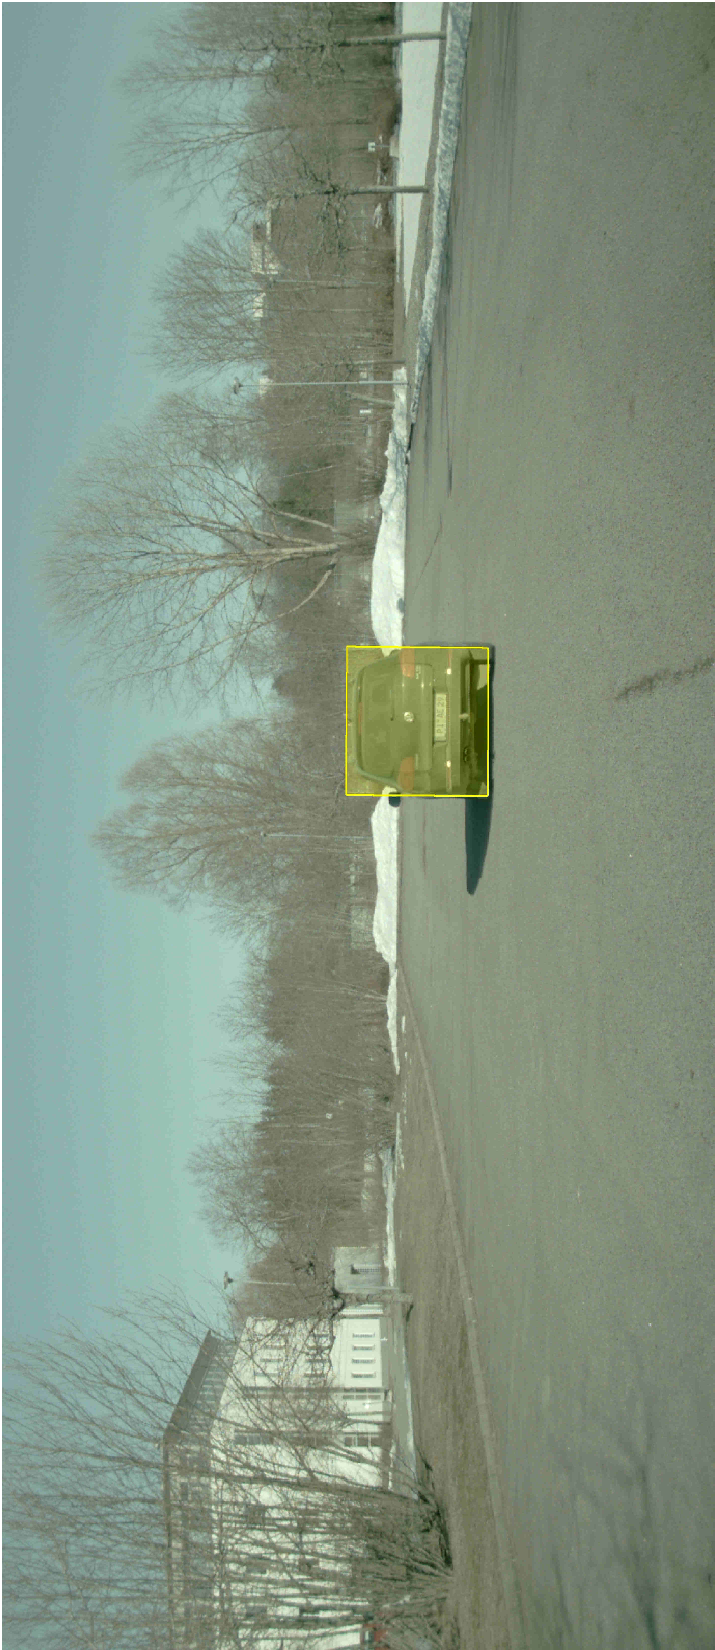
\includegraphics[angle=-90,origin=c,trim={0 0 15cm 0},width=0.9\textwidth]{roi_example}
	\caption{\label{fig:roiexample} An example of a vehicle that has been detected in a mono camera system using a classification appearance-based method. The vehicle has been marked by a box, referred to as the region of interest (\abbrROI).}
\end{figure}

\paragraph{Motion-based methods:}
Motion-based methods detect vehicles over a sequence of image frames.
Optical flow is one example of a method that can be used.
Optical flow is the motion of objects between frames, \ie how the pixels have moved from one frame to another.
The concept exists both as sparse optical flow, \ie the optical flow for a certain number of points in the image, and dense optical flow, \ie optical flow for all points in an image.

\subsection{Vehicle Tracking in Mono Camera Systems}
The goal of vehicle tracking is to predict and estimate \eg the position and velocity of the targets.
Many of the general object tracking aspects play an important role in vehicle tracking, \eg measurements, data association and \abbrMTT.
When tracking vehicles in a mono camera system, some alternatives are possible on how to select the states.
One can either track the vehicle in the image frame using image coordinates for position and velocity, or track in \spacedim{3} world coordinates and thus use meter and meter per second as units.
Since no depth information can be obtained from just a mono camera, some additional assumptions or other methods must be used if it is desired to track the target in \spacedim{3} world coordinates.

One of the main purposes of vehicle tracking is to maintain a state estimate of a vehicle even if it is not detected in a certain frame.
The tracking can \eg be performed with a filter of Kalman filter \cite{Sivaraman:2013} type.

\section{Related Research}
\label{sec:relatedresearch}
There exist several successful attempts of estimating the \spacedim{3} pose of objects using a mono camera system.
The problem of estimating the heading (including both the orientation and angular rate) of a vehicle can be seen as a special case of a full \spacedim{3} pose estimation problem.
A vehicle does not have the same degrees of freedom since it has limited rotational freedom.
\Figureref{fig:vehiclerotation} shows the rotation of interest, \ie the rotation around the axis which is perpendicular to the vehicle's ground plane.
Some different approaches found in the literature will be mentioned here.

\begin{figure}[!ht]
	\centering
	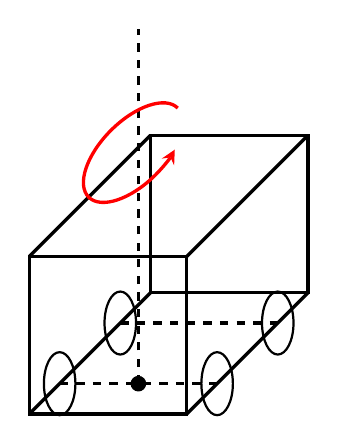
\begin{tikzpicture}
		[cube/.style={very thick,black}, wheel/.style={thick,black}]

		%draw the top and bottom of the cube
		\draw[cube] (0,0,0) -- (0,2,0) -- (2,2,0) -- (2,0,0) -- cycle;
		\draw[cube] (0,0,4) -- (0,2,4) -- (2,2,4) -- (2,0,4) -- cycle;

		%draw the edges of the cube
		\draw[cube] (0,0,0) -- (0,0,4);
		\draw[cube] (0,2,0) -- (0,2,4);
		\draw[cube] (2,0,0) -- (2,0,4);
		\draw[cube] (2,2,0) -- (2,2,4);

		\draw[wheel] (2,0,3) ellipse (0.2cm and 0.4cm);
		\draw[wheel] (0,0,3) ellipse (0.2cm and 0.4cm);
		\draw[wheel] (0,0,1) ellipse (0.2cm and 0.4cm);
		\draw[wheel] (2,0,1) ellipse (0.2cm and 0.4cm);

		%draw wheel axis
		\draw[cube, dashed] (0,0,3) -- (2,0,3);
		\draw[cube, dashed] (0,0,1) -- (2,0,1);

		\draw[cube, dashed] (1,0,3) node[circle,fill,inner sep=2pt] {} -- (1,4.5,3);
		%\draw[thick,dashed,red,->] (1,3,3) arc[x radius = 0.5cm, y radius = 0.75cm, start angle = 0, end angle = 180];
		\draw[very thick,red,->,>=stealth,rotate around={45:(1.5,3.5,3)}] (1.5,3.5,3) arc (0:300:0.8cm and 0.4cm);
		%\draw[thick,dashed,red,rotate around={-35:(1,3,3)}] (1,3,3) circle (0.5cm and 0.75cm);
	\end{tikzpicture}
	\caption{\label{fig:vehiclerotation} An illustration of which axis rotation that is of interest to estimate for a vehicle.}
\end{figure}

One straightforward way of estimating the \spacedim{3} pose of an object is to track a number of feature points over time and let an extended Kalman filter (\abbrEKF) estimate the rotation and translation parameters \cite{Hajimolahoseini:2014}.
By including the projection from \spacedim{3} to \spacedim{2}, the \abbrEKF estimates all necessary states directly.
No extra step to deal with the image projection is necessary.
The drawback is that the initial \spacedim{3} coordinates of the feature points must be known to a certain degree, which can be difficult to obtain from just a single image.
This method utilizes only image coordinates from the selected feature points as measurements.

In \cite{Blostein:2000}, another approach of estimating the \spacedim{3} pose is proposed.
Here, the \spacedim{3} trajectory and object structure are recovered from a sequence of images.
Especially, the optical flow for each selected feature point is utilized to improve the estimate instead of just using the image coordinates of feature points.
The usage of quaternions can be questioned, but might be good if the tracked object rotates in all three degrees of freedoms.
Using quaternions avoids the gimbal lock, which can occur when the pitch angle approaches 90 degrees \cite{Gustafsson:2012}.

Using the concept of homographies, \ie to estimate how planes have transformed between frames, is another concept, utilized in \cite{Gabb:2013}.
Here, the homography is estimated between frames in order to create a measurement of the angular rate of the target vehicle.
This method relies on having good correspondence between feature points in consecutive frames.
The Kanade-Lucas-Tomasi (\abbrKLT) feature tracker, \eg \cite{Szeliski:2011}, were used to track feature correspondences, between image frames.
The constructed measurement was used together with an \abbrEKF to obtain the state estimates.

In \cite{Mondragon:2010}, the homography concept is used in a somewhat similar manner.
Here, the yaw angle of an unmanned aerial vehicle (\abbrUAV) is estimated by calculating the homographies over time.
A helipad is placed on the ground as a reference plane onto which the homography is estimated.
Two flight tests were presented, and the resulting root-mean-square error (\abbrRMSE) of the yaw angle were $2.5^\circ$ and $4.9^\circ$, respectively.
A IMU was used as ground truth data.

\section{Coordinate Systems}
To describe tracking targets from a host, referring to the host as the ego car in which the camera system is located, some terminology about different coordinate systems is necessary.
First, we have the difference between a world coordinate system  and an image coordinate system.
A world coordinate system is a coordinate system in \spacedim{3} representing how objects are positioned in the world.
An image coordinate system is the \spacedim{3} world coordinates projected onto a \spacedim{2} image plane.

\vspace{1em}

The image coordinate system is defined in \Figureref{fig:imagecoordsystem}.
It is used to \eg express measurements from a mono camera system.

Two world coordinate systems are defined and used in this thesis: the target's coordinate system and the host's coordinate system.
The states of the tracked target will be expressed in both the host's world coordinate system and the target's world coordinate system.
They are defined in \Figuresref{fig:hostcoordsystem} and \ref{fig:targetcoordsystem}, respectively.

\vspace{4em}

\begin{figure}[!ht]
	\centering
	\begin{tikzpicture}
		\node [draw,circle,fill,inner sep=1pt] (origin) at (-3,2) {};
		\draw (origin.center) -- (-3,-2) -- (3,-2) -- (3,2)  -- cycle;
		\draw[very thick,->] (origin) -- (-1,2) node[anchor=south] {$u$};
		\draw[very thick,->] (origin) -- (-3,0) node[anchor=east] {$v$};
	\end{tikzpicture}
	\caption{\label{fig:imagecoordsystem} The definition of the image coordinate system. The origin is located in the upper left corner.}
\end{figure}

\vfill

\begin{figure}[!ht]
    \centering
    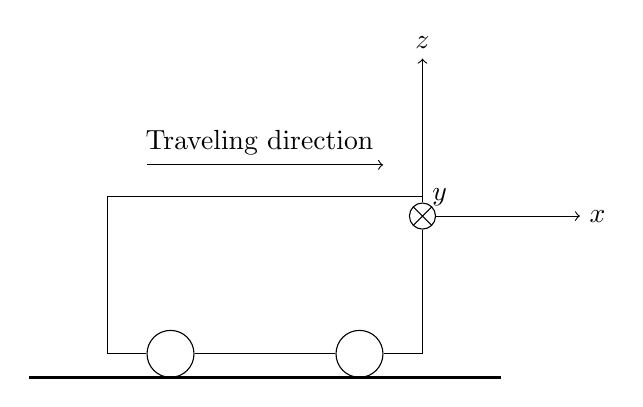
\begin{tikzpicture}
    [cross/.style={path picture={
		\draw[black]
			(path picture bounding box.south east) -- (path picture bounding box.north west) (path picture bounding box.south west) -- (path picture bounding box.north east);
	}}]
		\node [draw,circle,cross,minimum width=0.1 cm](origo) at (2, 0.75) {};
		\node [draw,circle,inner sep=6pt] (wheela) at (-1.2,-1) {};
		\node [draw,circle,inner sep=6pt] (wheelb) at (1.2,-1) {};

		\draw (-2,-1) -- (wheela) -- (wheelb) -- (2,-1) -- (origo) -- (2,1) -- (-2,1) -- (-2,-1);
		\draw[thick] (-3,-1.3) -- (3,-1.3);
		\draw[->] (origo) node[anchor=south west] {$y$} -- (4, 0.75) node[anchor=west] {$x$};
		\draw[->] (origo) -- (2, 2.75) node[anchor=south] {$z$};

		\draw[->] (-1.5, 1.4) -- (1.5, 1.4) node[anchor=south east] {Traveling direction};
    \end{tikzpicture}
    \caption{\label{fig:hostcoordsystem} The definition of the host's coordinate system. The coordinate system is placed at the height of the mounted camera system with the origin placed at the principal point of the camera. The $x$-direction points in the same direction as the host itself, the $y$-direction points to the left when looking in the host's direction and the $z$-direction points upwards.}
\end{figure}

\begin{figure}[!ht]
    \centering
    \hspace*{2cm}
    \begin{tikzpicture}[scale=0.95, every node/.style={scale=0.95}]
		\node [draw,circle,inner sep=3pt] (origo) at (0,-1) {};
		\draw (-1.5,-2) rectangle (1.5,2);
		\draw[dashed] (-1.5,-1) -- (1.5,-1) node[pos=0.5,circle,fill,inner sep=1pt] {};
		\draw[->] (origo) node[anchor=north west] {$z$} -- (0,1) node[anchor=south] {$x$};
		\draw[->] (origo) -- (-2,-1) node[anchor=east] {$y$};
		\draw[->] (1.9,-1.5) -- (1.9,1.5) node[pos=0.5, anchor=west] {Traveling direction};
    \end{tikzpicture}
    \caption{\label{fig:targetcoordsystem} The definition of the target's coordinate system. The coordinate system is placed at the center of the rear axis of the target. The $x$-direction points in the same direction as the target itself, the $y$-direction  points to the left when looking in the target's direction and the $z$-direction points upwards.}
\end{figure}

\newpage

\section{The Pinhole Camera Model}
One basic camera model is the pinhole camera model \cite{Hartley:2004}.
It describes how a point in world coordinates projects onto the image coordinate system.
\Figureref{fig:pinholecameraex} illustrates how a point $(x, y, z)^T$ is mapped onto the image plane.
If the camera has the focal lengths $f_u$ and $f_v$, and by identifying similar triangles, the resulting mapping from \spacedim{3} to \spacedim{2} is
\begin{subequations}
\begin{equation}
    (x, y, z)^T \mapsto \left(f_u\frac{y}{x}, f_v\frac{z}{x}\right)^T,
\end{equation}
\ie
\begin{equation}
    (u, v)^T \mapsto \left(f_u\frac{y}{x}, f_v\frac{z}{x}\right)^T.
\end{equation}
\end{subequations}

\begin{figure}[!ht]
	\centering
	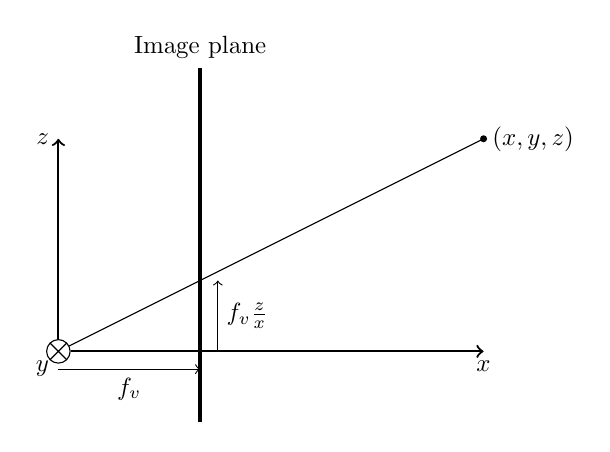
\begin{tikzpicture}
		[scale=0.9, every node/.style={scale=0.9},
		axis/.style={thick,black,->},
		 cross/.style={path picture={
			\draw[black]
			(path picture bounding box.south east) -- (path picture bounding box.north west) (path picture bounding box.south west) -- 			(path picture bounding box.north east);}}]
		\node [draw,circle,cross,minimum width=0.1 cm] (origin) at (0,0) {};
		\coordinate (xaxis) at (6,0);
		\coordinate (zaxis) at (0,3);

		% Coordinate axis
		\draw[axis] (origin) node[anchor=north east] {$y$} -- (xaxis) node[anchor=north] {$x$};
		\draw[axis] (origin) -- (zaxis) node[anchor=east] {$z$};

		% Image plane
		\draw[very thick] (2,-1) -- (2,4) node[anchor=south] {Image plane};

		% 3D coordinate
		\draw[] (origin) -- (6,3) node[anchor=west] {$(x,y,z)$} node[circle,fill,inner sep=1pt] {};
		
		% Focal axis
		\draw[->] (0,-0.25) -- (2,-0.25) node[pos=0.5,anchor=north] {$f_v$};

		% Projected size in image
		\draw[->] (2.25,0) -- (2.25, 1) node[pos=0.5,anchor=west] {$f_v \frac{z}{x}$};
	\end{tikzpicture}
	\caption{\label{fig:pinholecameraex} A world coordinate $(x, y, z)^T$ is projected onto the image plane. The figure shows the similar triangles for the projection in the $v$-direction.}
\end{figure}

\section{Homography}
\label{sec:homography}
The homography is a projective transformation.
The exact definition and more about projective transformations can be found in \eg \cite{Hartley:2004}, more precisely as Definitions 2.9 and 2.11, and Theorem 2.10.
Definition 2.11 from \cite{Hartley:2004} is of special interest, so it is recapitulated here and referred to as \Definitionref{def:projtrans}.

\begin{definition}[Projective transformation] \label{def:projtrans}
	A planar projective transformation is a linear transformation on homogeneous \spacedim{3} vectors represented by a nonsingular $3 \times 3$ matrix:
	\begin{equation}
		\begin{pmatrix} x^\prime_1 \\ x^\prime_2 \\ x^\prime_3 \end{pmatrix}
		=
		\begin{pmatrix}
			h_{11} & h_{12} & h_{13} \\
			h_{21} & h_{22} & h_{23} \\
			h_{31} & h_{32} & h_{33}
		\end{pmatrix}
		\begin{pmatrix} x_1 \\ x_2 \\ x_3 \end{pmatrix},
	\end{equation}
	or in short, $\bm{x}^\prime = \bm{H} \bm{x}$.
\end{definition}
%
As described in \cite{Nordberg:2015}, any nonzero scalar multiplied into $\bm{H}$ is also a representative of the same homography.
The projective transformation can therefore be formulated as
%
\begin{subequations}
\begin{equation}
	\label{eq:homography}
	\bm{x}^\prime \sim \bm{H} \bm{x},
\end{equation}
%
or by using an equality sign,
%
\begin{equation}
	\label{eq:homographyequality}
	\gamma \bm{x}^\prime = \bm{H} \bm{x},
\end{equation}
\end{subequations}
%
for some nonzero scalar $\gamma$.
One example of how a projective transformation can be used, mentioned in \cite{Hartley:2004}, is mapping between planes. 
This is the idea used in \cite{Gabb:2013} to estimate the angular rate of vehicles and in \cite{Mondragon:2010} to estimate the yaw angle of a \abbrUAV.

The problem of estimating how a plane in \spacedim{3}, given a set of image coordinates $\bm{x}_i \in \mathbb{P}^2$ and a corresponding set of image coordinates $\bm{x}^\prime_i \in \mathbb{P}^2$, has moved (translated and rotated) between two frames is equivalent to finding the homography $\bm{H}$ for the two correspondence set of homogeneous image coordinates $\bm{x} = (u_i, v_i, 1)^T$ and $\bm{x}^\prime = (u^\prime_i, v^\prime_i, 1)^T$.
The interpretation of corresponding points is a point before and the same point after the homography transformation.
There exist several methods for finding the homography from the corresponding points.

\subsection{Direct Linear Transform}
The homography matrix, $\bm{H}$, can be estimated given a set of $N$ image coordinates, $\bm{x}_i = (u_i, v_i, 1)^T$, and the correspondence set of $N$ image coordinates, $\bm{x}^\prime_i = (u^\prime_i, v^\prime_i, 1)^T$, in another frame.

By rewriting \eqref{eq:homographyequality}, and by substituting the third row, $\gamma_i = h_{31}u_i + h_{32}v_i + h_{33}$, into the other two rows, a resulting linear equation system on the form
%
\begin{equation}
	\label{eq:geoerrorhomography}
	\bm{A} \bm{h} = \bm{0}
\end{equation}

\vspace{1em}

is obtained and is referred to as a direct linear transformation (\abbrDLT), \eg \cite{Hartley:2004} and \cite{Nordberg:2015}, where $\bm{A}$ is a $2 N \times 9$ matrix and $\bm{h}$ is a $9 \times 1$ vector,
%
\begin{equation}
	\bm{A} =
	\begin{pmatrix}
		u_1 & 0 & -u_1 u_1^\prime & v_1 & 0 & - v_1 u_1^\prime & 1 & 0 & -u_1^\prime \\
		0 & u_1 & -u_1 v_1^\prime & 0 & v_1 & - v_1 v_1^\prime & 0 & 1 & -v_1^\prime \\
		\vdots & \vdots & \vdots & \vdots & \vdots & \vdots & \vdots & \vdots & \vdots \\
		u_N & 0 & -u_N u_N^\prime & v_N & 0 & - v_N u_N^\prime & 1 & 0 & -u_N^\prime \\
		0 & u_N & -u_N v_N^\prime & 0 & v_N & - v_N v_N^\prime & 0 & 1 & -v_N^\prime
	\end{pmatrix}
	,
	\quad
	\bm{h} =
	\begin{pmatrix}
		h_{11} \\
		h_{21} \\
		h_{31} \\
		h_{12} \\
		h_{22} \\
		h_{32} \\
		h_{13} \\
		h_{23} \\
		h_{33} \\
	\end{pmatrix}
	.
\end{equation}
%
Viewing \eqref{eq:geoerrorhomography} as a least squares problem, turns \eqref{eq:geoerrorhomography} into the optimization problem
%
\begin{equation}
	\min_{\bm{h}} \sum_i
	\left( u^\prime_i - \frac{h_{11}u_i + h_{12}v_i + h_{13}}{h_{31}u_i + h_{32}v_i + h_{33}} \right)^2 +
	\left( v^\prime_i - \frac{h_{21}u_i + h_{22}v_i + h_{23}}{h_{31}u_i + h_{32}v_i + h_{33}} \right)^2.
\end{equation}

\subsection{Random Sample Consensus}
\label{sec:ransac}
If the data contains outliers, the \abbrDLT solution generally results in a bad estimate.
Since all data points have equal weights, outliers, \ie points that do not fit the estimated model, can have significant impact on the estimation result.
Random sample consensus (\abbrRANSAC), \eg \cite{Hartley:2004} and \cite{Nordberg:2015}, is one method which can improve the result if the data set contains outliers.
The method contains some tuning parameters selected by the user.
Some notable notations used in the algorithm are:

\begin{description}[align=left,labelwidth=3cm,noitemsep]
	\item [Trial set $T$] A random subset of the total data set.
	\item [Consensus set $\bm{C}$] All data points satisfying the homography estimated from $T$.
	\item [Threshold $t$] Determines if a corresponding point pair belongs to $\bm{C}$ or not.
	\item [Number of trials $r$] The number of times a trial set $T$ is selected.
\end{description}

The complete algorithm with all details can be found in \cite{Nordberg:2015}.
Here, a brief overview of the algorithm is provided in \Algorithmref{algo:ransach}.

\begin{algorithm}[!ht]
	\caption{\label{algo:ransach} A \abbrRANSAC algorithm for estimating the homography}
	\begin{algorithmic}
		\State \textbf{input} data set $D$, threshold $t$, number of trials $r$
		\State Initialize $\bm{H}_\text{est} = \emptyset$ and $\bm{C}_\text{est} = \emptyset$
		\While {$i = \{1,\dots,r\}$}
			\State Pick a random subset $T$ with 4 pairs of corresponding points from $D$
			\State Determine $\bm{H}$ from $T$ using the \abbrDLT method
			\State Initialize $\bm{C} = \emptyset$
			\ForAll {point pair $\{\bm{x}^\prime, \bm{x}\}$ in the data sets $D$}
				\State Compute an error $\epsilon$, measuring how well $\{\bm{x}^\prime, \bm{x}\}$ fits $\bm{H}$
				\If {$\epsilon < t$}
					\State Add $\{\bm{x}^\prime, \bm{x}\}$ to $\bm{C}$
				\EndIf
			\EndFor
			\If {size of $\bm{C}$ is larger than size of $\bm{C}_\text{est}$}
				\State Set $\bm{H}_\text{est} = \bm{H}$ and $\bm{C}_\text{est} = \bm{C}$
			\EndIf
		\EndWhile
		\State \Return $\bm{H}_\text{est}$ and $\bm{C}_\text{est}$
	\end{algorithmic}
\end{algorithm}

\clearpage

\section{Feature Points}
In order to get the corresponding image coordinates, mentioned in \Sectionref{sec:homography}, and the optical flow, mentioned in \Sectionref{sec:objectdetection}, a selection of certain points from the image, referred to as feature points, has to be done.
An example of detected feature points in an image can be seen in \Figureref{fig:featurepointexample}.
There exist mainly three different steps, where the last step can be performed in two ways, when detecting feature points and finding the correspondence between images \cite{Szeliski:2011}.
They are:

\begin{description}[align=left,labelwidth=3cm]
	\item [Feature detection] Find and extract image points that are easily recognisable and distinguishable from its surroundings. Typically, this means points that have a large image gradient.
	\item [Feature description] A descriptor is an alternative representation of the image point. Its purpose is to be a robust description of the feature point and its surrounding region. Examples of descriptors are: Scale-invariant feature transform (SIFT) and gradient location and orientation histogram (GLOH) \cite{Szeliski:2011}.
	\item [Feature matching] Feature points are separately extracted from two consecutive images and then the descriptors are compared in order to matched points between the two images.
	\item [Feature tracking] Instead of matching extracted feature points between two images, one can in the second frame search for the feature points detected in the first frame, \ie track the feature points. The \abbrKLT tracker is a popular feature point tracker.
\end{description}

\begin{figure}[!ht]
	\centering
	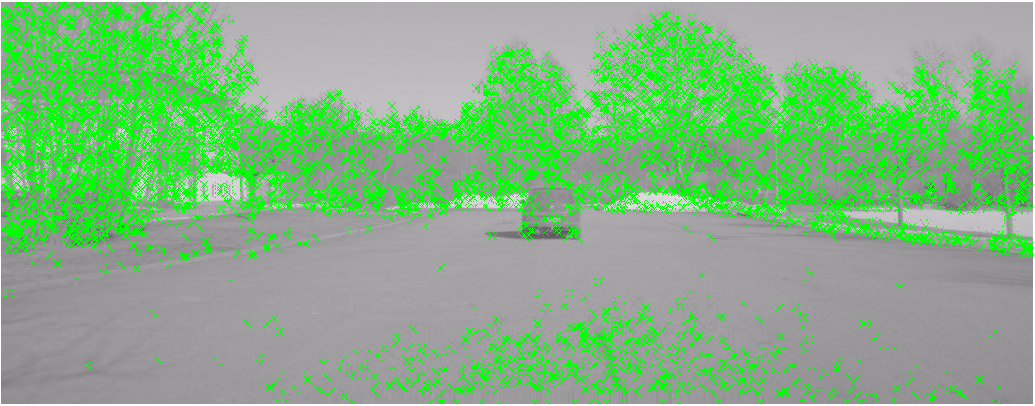
\includegraphics[width=0.9\textwidth]{155532_harris_features}
	\caption{\label{fig:featurepointexample} An example of an image with detected feature points marked as green crosses. Here, the Harris–Stephens corner detection algorithm \cite{Harris:1988} was used to detect interesting points.}
\end{figure}

\newpage

\section{Extended Kalman Filtering}
Kalman filtering \cite{Gustafsson:2012} is one filtering method used to track a target.
If the target is moving according to some motion model, $\bm{f}(\bm{x}_k,\bm{u}_k,\bm{v}_k)$, and measurements are generated according to some measurement model, $\bm{h}(\bm{x}_k,\bm{u}_k,\bm{e}_k)$, the system is described by
\begin{align}
\begin{split}
	\bm{x}_{k+1} &= \bm{f}(\bm{x}_k,\bm{u}_k,\bm{v}_k), \\
	\bm{y}_k &= \bm{h}(\bm{x}_k,\bm{u}_k,\bm{e}_k).
\end{split}
\end{align}
Here, $\bm{x}_k$ is the state of the target, $\bm{u}_k$ is an input or control signal to the system, $\bm{v}_k$ is the process noise and $\bm{e}_k$ is the measurement noise.
The process and measurement noise are assumed to be Gaussian with zero mean and covariance matrices denoted $\bm{Q}$ and $\bm{R}$, respectively.
The motion and measurement models used in this thesis are nonlinear, thus the \abbrEKF can be applied.
The algorithm to perform \abbrEKF filtering can be found in \cite{Gustafsson:2012} and is recapitulated in \Algorithmref{algo:ekf}.
In the algorithm outline, the input signal $\bm{u}_k$ has been omitted.

\begin{algorithm}
	\caption{\label{algo:ekf} Extended Kalman filtering algorithm}
	Given some initial conditions, $\hat{\bm{x}}_{1|0}$ and $\bm{P}_{1|0}$, the \abbrEKF solves the filtering problem by a, two step, recursion algorithm. \\ \\
	\begin{subequations}
	Measurement update:
	\begin{align}
		\bm{S}_k &= \bm{R}_k + \bm{h}^\prime(\hat{\bm{x}}_ {k|k-1}) \bm{P}_{k|k-1} (\bm{h}^\prime(\hat{\bm{x}}_ {k|k-1}))^T \\
		\bm{K}_k &= \bm{P}_{k|k-1} (\bm{h}^\prime(\hat{\bm{x}}_ {k|k-1}))^T \bm{S}_k^{-1} \\
		\bm{\epsilon}_k &= \bm{y}_k - \bm{h}(\hat{\bm{x}}_{k|k-1}) \\
		\hat{\bm{x}}_{k|k} &= \hat{\bm{x}}_{k|k-1} + \bm{K}_k \bm{\epsilon}_k \\
		\bm{P}_{k|k} &= \bm{P}_{k|k-1} - \bm{K}_k \bm{h}^\prime(\hat{\bm{x}}_{k|k-1}) \bm{P}_{k|k-1}
	\end{align}
	\\
	Time update:
	\begin{align}
		\hat{\bm{x}}_{k+1|k} &= \bm{f}(\hat{\bm{x}}_{k|k}) \\
		\bm{P}_{k+1|k} &= \bm{Q}_k + \bm{f}^\prime(\hat{\bm{x}}_{k|k}) \bm{P}_{k|k} (\bm{f}^\prime(\hat{\bm{x}}_{k|k}))^T
	\end{align}
	\end{subequations}
\end{algorithm}

Here, $\bm{f}^\prime(\hat{\bm{x}}_k)$ and $\bm{h}^\prime(\hat{\bm{x}}_k)$ are the Jacobians of $\bm{f}(\hat{\bm{x}}_k)$ and $\bm{h}(\hat{\bm{x}}_k)$, respectively.
The matrices $\bm{R}_k$ and $\bm{Q}_k$ are the covariance matrices of $\bm{e}_k$ and $\bm{v}_k$, respectively.
The algorithm is based on the first order moment Taylor expansion.

\section{Observability Analysis}
\label{sec:obsanalysis}
To be able to estimate the state $\bm{x}_k$, from the available measurements, the system must be observable.
For a system on linear state-space form,
\begin{align}
\label{eq:linearss}
\begin{split}
	\bm{x}_{k+1} &= \bm{A}_k \bm{x}_k + \bm{B}_k \bm{u}_k, \\
	\bm{y}_k &= \bm{C}_k \bm{x}_k + \bm{D}_k \bm{u}_k,
\end{split}
\end{align}
the observability can be determined using the observability Gramian \cite{Rugh:1996}.
Recalling the definition of observability from \cite{Rugh:1996}, which gives \Definitionref{def:observability}.

\begin{definition}[Observability] \label{def:observability}
	The linear state-space model \eqref{eq:linearss} is observable in the interval $[t_0, t_N]$ if any initial state $\bm{x}_0$ is uniquely determined by the corresponding zero-input response $\bm{y}_k$ for $k=t_0,\dots,t_N-1$.
\end{definition}

The condition for having an observable linear state equation is given by \Theoremref{th:observability} from \cite{Rugh:1996}.
%
\begin{theorem}
\label{th:observability}
	The linear state equation \eqref{eq:linearss} is observable on $[t_0, t_N]$ if and only if the $n \times n$ matrix
	\begin{equation}
	\label{eq:observabilitytheorem}
		\bm{M}(t_0,t_N) = \sum_{j=t_0}^{t_N-1} \bm{\Phi}^T(j,t_0)\bm{C}^T_j\bm{C}_j\bm{\Phi}(j,t_0)
	\end{equation}
	is invertible.
\end{theorem}
%
Here, the matrix $\bm{M}$ is the observability Gramian and $\bm{\Phi}$ is the transition matrix, which is, for $k \ge j$, given by
%
\begin{equation}
	\bm{\Phi}(k,j) =
		\begin{cases}
			\bm{A}_{k-1} \bm{A}_{k-2} \cdots \bm{A}_j & \text{if } k \ge j+1, \\
			\bm{I} & \text{if } k = j.
		\end{cases}
\end{equation}
%
In the case of a nonlinear state-space model,
%
\begin{align}
\label{eq:nlss}
\begin{split}
	\bm{x}_{k+1} &= \bm{f}(\bm{x}_k), \\
	\bm{y}_k &= \bm{h}(\bm{x}_k),
\end{split}
\end{align}
%
where the control signal $\bm{u}_k$ has been omitted, the state-space model first has to be linearized.
By linearizing using a Taylor expansion and retaining only the first order terms, the resulting linearized state-space model is
%
\begin{equation}
\begin{split}
	\bar{\bm{x}}_{k+1} = \bm{f}^\prime(\bm{\tilde{\bm{x}}_k}) \bar{\bm{x}}_k, \\
	\bar{\bm{y}}_{k} = \bm{h}^\prime(\bm{\tilde{\bm{x}}_k}) \bar{\bm{x}}_k,
\end{split}
\end{equation}
%
where $\bm{x}_k = \tilde{\bm{x}}_k + \bar{\bm{x}}_k$ and $\tilde{\bm{x}}_k$ is the point around which the Taylor expansion took place, the matrix $\bm{f}^\prime(\bm{\tilde{\bm{x}}_k})$ is the Jacobian of $\bm{f}(\bm{x}_k)$ and $\bm{h}^\prime(\bm{\tilde{\bm{x}}_k})$ is the Jacobian of $\bm{h}(\bm{x}_k)$, respectively.
The model now fits into the structure of \Definitionref{def:observability} and \Theoremref{th:observability}.
